
\subsubsection{Interfaces Cerebro-Computador (BCI)}

Definición → 1 párrafo
Funcionamiento + figura → 2 párrafos
Aplicaciones → 1 párrafo
Tipos → 1 párrafo


Una interfaz cerebro-computador (BCI) es un sistema capaz de adquirir señales cerebrales, procesarlas y traducirlas en comandos de control para un dispositivo externo, sin necesidad de utilizar las vías motoras convencionales \cite{young_BraincomputerInterfaces2021,he_BrainComputer2020}. Inicialmente, las aplicaciones de estas interfaces se centraban en la rehabilitación y asistencia médica para la recuperación de capacidades motoras de pacientes con lesiones motoras\cite{,waldert_InvasiveVs2016,he_BrainComputer2020}.

El esquema general de las \acrshort{bci} se representa en la figura \ref{fig:esquemaBCI}. En él se observan las distintas fases de las que se compone el sistema de control. El primer paso es la adquisición de la señal cerebral, en el cual se registran los potenciales mediante electrodos posicionados en distintas zonas de la cabeza\cite{wolpaw_BraincomputerInterfaces2012}. 

Después de la adquisición de la señal, se realiza un paso intermedio en el cual se eliminan posibles artefactos de la señal, como las interferencias de red o las componentes de ruido.

A continuación estas señales son procesadas para extraer las características específicas sujeto de análisis. Es procesamiento incluye uno o varios métodos de filtrado, como el análisis espectral, la medición de la amplitud de voltajes, etc. Este 


Se trata de una tecnología capaz de ayudar en la rehabilitación de pacientes con lesiones motoras, al igual que permite reemplazar las funciones de los miembros dañados por la lesión en pacientes crónicos\cite{he_BrainComputer2020}.

The immediate goal is to provide these users, who may be completely paralyzed, or ‘locked in’, with basic communication capabilities so that they can express their wishes to caregivers or even operate word processing programs or neuroprostheses\cite{wolpaw_BrainComputer2002}.


A BCI output might replace natural output that has been lost as a result of injury or disease. For example, a person who can no longer speak might use a BCI to type words that are then spoken by a speech synthesizer. Or a person who has lost limb control might use a BCI to operate a motorized wheelchair. In these examples the BCI outputs replace lost natural outputs.  A BCI output might restore lost natural output. For example, a person with spinal cord injury whose arms and hands are paralyzed might use a BCI to stimulate the paralyzed  muscles via implanted electrodes so that the muscles move the limbs. Or a person who has lost bladder function due to multiple sclerosis might use a BCI to stimulate the peripheral nerves that control the bladder, thus enabling urination. In these examples, the BCI outputs restore the natural outputs.  A BCI output might enhance natural CNS output. For example, a person performing a task that requires continuous attention over a prolonged period (e.g., driving a vehicle or serving as a sentry) might use a BCI that detects the brain activity preceding lapses in attention and then provides an output (e.g., a sound) that alerts the person and restores attention. By preventing the attentional lapses that periodically impair natural CNS output (and might cause traffic accidents), the BCI enhances the natural output.  A BCI output might supplement natural CNS output. For example, a person who is controlling the position of a computer cursor with a hand-operated joystick might use a BCI to select items that the cursor reaches. Or a person might use a BCI to control a third (i.e., robotic) arm and hand. In these cases, the BCI supplements natural neuromuscular output with an additional, artificial output \cite{wolpaw_BraincomputerInterfaces2012}.


{
    \color{red}{
        El funcionamiento general de una BMI está representado en la Figura 4. El primer paso,  es la adquisición de los datos, donde las señales cerebrales del sujeto son registradas mediante electrodos, invasivos o no invasivos, ubicados en su cabeza y transformadas a señales digitales a través de amplificadores.  El segundo paso, es el procesamiento de las señales registradas aplicándoles una serie de filtros para eliminar ruido y otros artefactos, como las interferencias de red. Una vez acondicionada la señal, el tercer paso es extraer características de los trozos de señal y se  seleccionan aquellas que aportan información relevante para diferenciar la tarea en el clasificador.  El siguiente paso es clasificar los ritmos motores captados por los electrodos según los potenciales evocados o intenciones motoras que puedan contener. En función de la clasificación de la señal, se producen distintos comandos de control en otros dispositivos,  como pueden ser ordenadores, robots domésticos o exoesqueletos, entre otros. Tras ejecutar el comando, el dispositivo que lo ha ejecutado produce una respuesta que es transmitida al sujeto.  Generalmente, los BMI son sistemas de bucle cerrado donde el sujeto es realimentado con información acerca del resultado de las órdenes enviadas al dispositivo. La respuesta recibida varía dependiendo del dispositivo al que está vinculado la BMI. Cuando está  conectada a un ordenador recibirá un feedback visual. En cambio, cuando se trate de un exoesqueleto, la respuesta será a través de un movimiento en la extremidad del sujeto

        En primer lugar, los BMI invasivos consisten en introducir los electrodos en la región intracortical de la cabeza. Este procedimiento implica una operación donde se retira un trozo de cráneo para implantar los electrodos en el cerebro y pinchar las neuronas. La  principal ventaja de esta técnica es que la adquisición de la señal se hace directamente sobre las neuronas que producen las señales deseadas. Por tanto, la señal tiene una gran resolución espacial y temporal con escaso ruido. Sin embargo, esta técnica presenta una importante desventaja que es exponer al paciente a una intervención quirúrgica compleja  y a electrodos en el interior de su cuerpo, que tarde o temprano deben ser o bien reemplazados, o bien retirados.  En segundo lugar, los BMI parcialmente invasivos colocan los electrodos sobre la superficie del cerebro. Esta técnica es muy similar a la anterior, pero en este caso la captación se realiza por electrocorticografía (ECoG) [15]. Este método presenta una resolución espacial y temporal medias, ya que eliminan parte de los artefactos causados  por la piel y el hueso, pero las señales de las regiones más profundas del cerebro siguen presentando una pequeña cantidad de ruido espacial. Por el contrario, la principal  Figura 9. Posición de los electrodos en la cabeza para la adquisición de las señales EEG. [4] 13 desventaja que presentan es exactamente la misma que en las BMI invasivas: la  intervención quirúrgica y sus riesgos. Adicionalmente, ambas técnicas implican un elevado coste.  En tercer lugar, los BMI no invasivos ubican los electrodos en la superficie de la cabeza, sobre el cuero cabelludo. Por tanto, se elimina el problema de someter al paciente a la cirugía y se reduce el coste. Además, los electrodos son portables, normalmente están  agrupados en un casco, y se puede colocar en distintos entornos, no sólo en un quirófano. Sin embrago, el tiempo de colocación de los electrodos es muy elevado. Asimismo, la desventaja de eliminar los electrodos no invasivos es que se pierde resolución espacial, especialmente al realizar la captación por EEG o MEG, donde algunos electrodos registran señales de múltiples regiones. No obstante, este método no pierde la resolución temporal
    }
}


\begin{figure}[htbp]
    \centering
    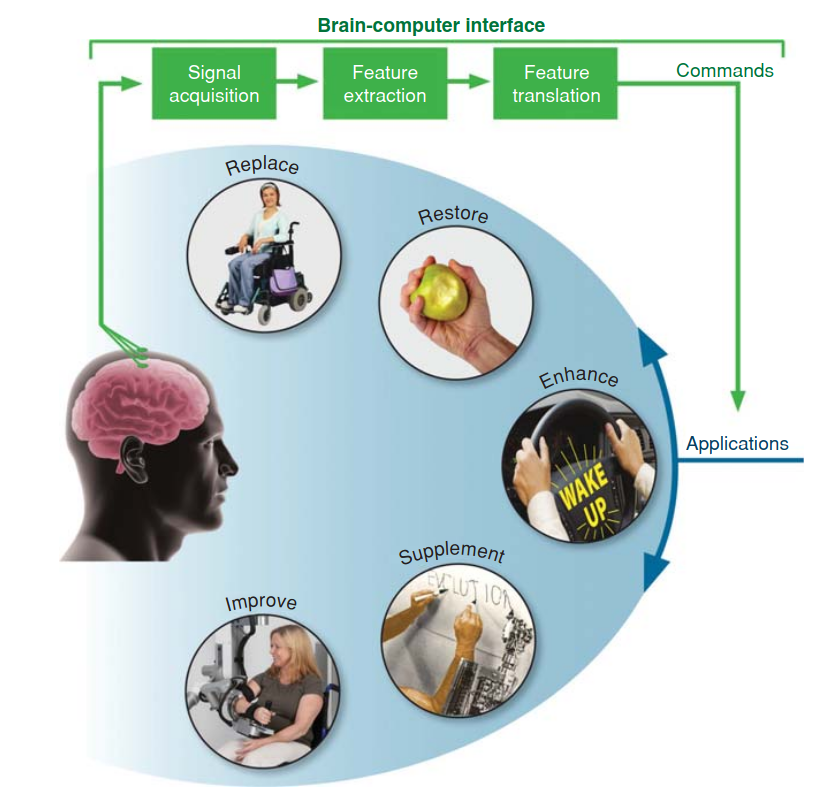
\includegraphics[width=0.90\textwidth]{img/bci_schema.png}
    %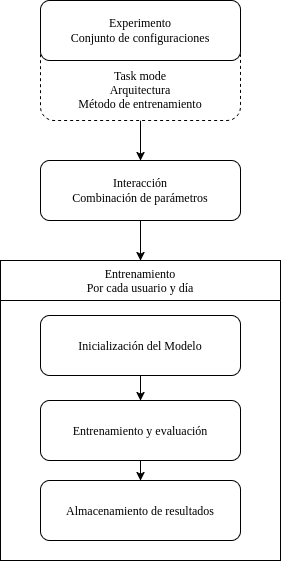
\includegraphics[height=\dimexpr\pagegoal-\pagetotal-\baselineskip\relax,width=\textwidth,keepaspectratio]{img/diagrama_pipeline.drawio.png}
    \caption{Esquema general del funcionamiento de una BCI \cite{wolpaw_BraincomputerInterfaces2012}}
    \label{fig:esquemaBCI}
\end{figure}


SACAR COSAS DE \cite{lawhern_EEGNetCompact2018}

{\color{red}
Como tecnología asistiva
Cuando el daño motor de un individuo ya es crónico, estas
interfaces se pueden utilizar como herramienta de comunicación,
para controlar miembros artificiales (sustitución motora) o incluso
para el ocio

Sustitución motora

• El concepto de movilidad asistiva se puede encuadrar dentro de la
sustitución motora
• Un ejemplo es el uso de sillas de ruedas controladas por BCI
• La silla de ruedas, es considerada, por muchos usuarios como
parte de su propio cuerpo (embodiment) y funciona de forma
equivalente a una prótesis}

\begin{figure}[H]
    \centering
    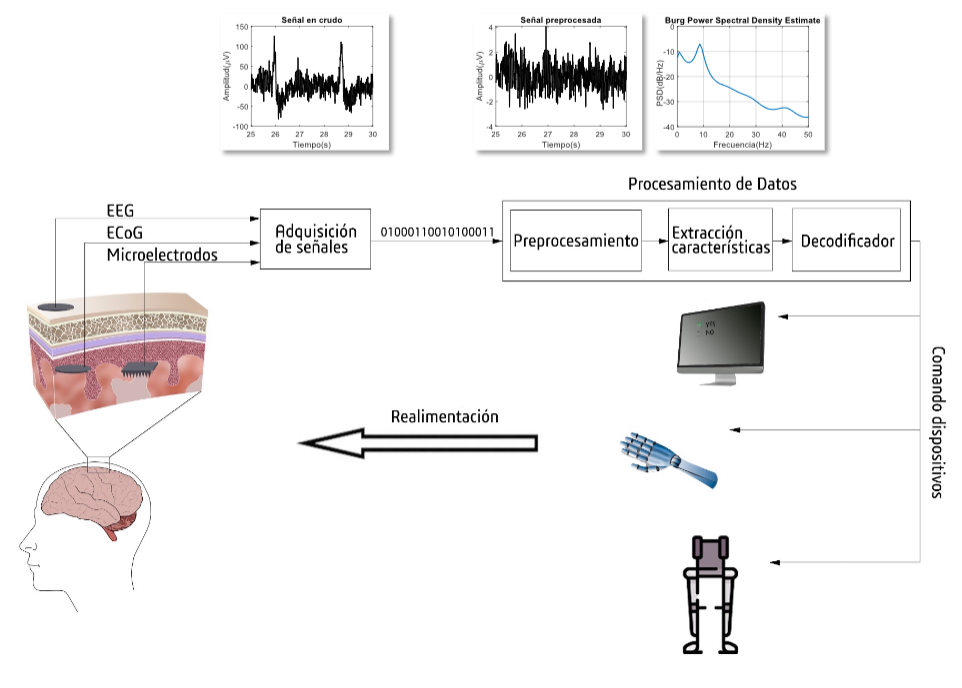
\includegraphics[width=0.90\textwidth]{img/esquema_bci.png}
    %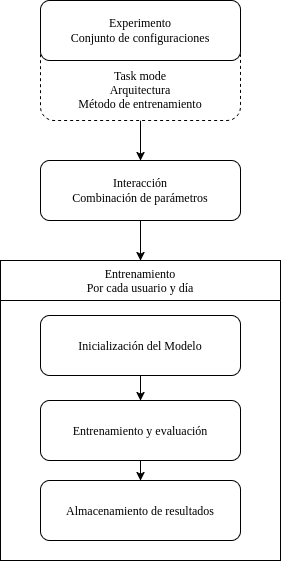
\includegraphics[height=\dimexpr\pagegoal-\pagetotal-\baselineskip\relax,width=\textwidth,keepaspectratio]{img/diagrama_pipeline.drawio.png}
    \caption{Esquema general de una BCI \cite{azorinpoveda_Tema322024}}
    \label{fig:pbci_esquema}
\end{figure}

\begin{comment}

    \begin{itemize}
    \item Qué es
    \item Pipeline típico:
    \begin{itemize}
    \item adquisición → preprocesado → clasificación → acción
\end{itemize}
\end{itemize}
\end{comment}


